% LaTeX Article Template - customizing page format
%
% LaTeX document uses 10-point fonts by default.  To use
% 11-point or 12-point fonts, use \documentclass[11pt]{article}
% or \documentclass[12pt]{article}.
\documentclass{article}

% Set left margin - The default is 1 inch, so the following 
% command sets a 1.25-inch left margin.
\setlength{\oddsidemargin}{0.25in}

% Set width of the text - What is left will be the right margin.
% In this case, right margin is 8.5in - 1.25in - 6in = 1.25in.
\setlength{\textwidth}{6in}

% Set top margin - The default is 1 inch, so the following 
% command sets a 0.75-inch top margin.
\setlength{\topmargin}{-0.25in}

% Set height of the text - What is left will be the bottom margin.
% In this case, bottom margin is 11in - 0.75in - 9.5in = 0.75in
\setlength{\textheight}{8in}
\usepackage{fancyhdr}
\usepackage{float}
\usepackage{mathtools}
\usepackage{amsmath}
\usepackage{amssymb}
\usepackage{graphicx}
\usepackage{float}
\usepackage{tikz}
\usetikzlibrary{positioning}
\graphicspath{ {./} }
\setlength{\parskip}{5pt} 
\pagestyle{fancyplain}

% Universes
\newcommand{\NN}{\mathbb{N}}
\newcommand{\ZZ}{\mathbb{Z}}
\newcommand{\QQ}{\mathbb{Q}}
\newcommand{\RR}{\mathbb{R}}
\newcommand{\CC}{\mathbb{C}}

% Groups commands
\newcommand{\inv}{^{-1}}
\newcommand{\lcm}{\mathrm{lcm}}
\newcommand{\lr}[1]{\langle #1 \rangle}
% Set the beginning of a LaTeX document
\begin{document}

\lhead{Drew Remmenga MATH 458}
\rhead{HW \#3}
%\lhead{Independent Study}
%\rhead{R Lab}
\begin{enumerate}
\item Let $G$ be an abelian group. (Do not assume that $G$ is finite.)
	\begin{enumerate}
	\item Prove that $H=\{x\in G\mid|x|\text{ is odd}\}$ is a subgroup of $G$. 
	It is clear that $H$ is finite as $G$ is finite. Here $H$ is non empty as $e\in H$ since the power of $e$ is one which is odd. Assume $a,b \in H$. This implies that there are odd integers p and q such that $a^{p} = e$ and $b^{q} = e$. Now consider the closure of $H$. $(a \circ b)^{pq} = a ^{pq} \circ b^{pq}$ since $G$ is abelian. Now we have $(a^{p})^{q} \circ (b^{q})^{p} = e$. The multiplication of two odd integers is odd so $a \circ b \in H$. Thus $H$ is closed. Hence $H$ is a subgroup of $G$. 
	\item Give an example to show that $K=\{x\in G\mid|x|\text{ is 1 or even}\}$ need not be subgroup of $G$. 
Consider the integers under addition modulo six. The set containing three has order one but does not contain the identity so it is not a subgroup.
	\end{enumerate} 
\item Show that $U(n)$ is a group under multiplication modulo $n$. 
	\begin{enumerate}
	\item Associativity: Associativity is inherited from the integers.
	\item Identity: 1 is always in $U(n)$ so $e$ =1.
	\item  Closure: Let $a,b \in U(n)$. $a$ has no common factor with $n$ (other than 1) $b$ has no common factor with $n$ (other than 1) So, If $ab < n$, then $ab$ doesn't have any common factors with $n$. If $ab>n$, then for some $p\in \ZZ$,$ab-pn < n$. Since $ab$ doesn't have any common factor with $n$, $ab-pn$ can't either. $ab \neq n$, because neither $a$ nor $b$ can have any common factors with $n$) So, $ab \in U(n)$
	\item Inverse:  Fix $a \in U(n)$. Because $gcd(a, n) = 1$, there exist integers $s, t \in \ZZ$ such that
$sa + tn = 1$. Working modulo $n$, we see that $sa \equiv 1 (mod n)$. But we have thus found our
inverse to $a$, namely $s mod n$.
	\end{enumerate}
    
    
    \item Find a noncyclic subgroup of order 4 in $U(36)$. \textit{(Hint: Use Homework 2 Problem 3 for inspiration.)}

${1,17,19,35}$
    

    \item Determine the subgroup lattice of $\ZZ_{16}$. Generalize to $\ZZ_{p^n}$ where $p$ is prime and $n$ is some positive integer. (No justification required.)
    
    %%%% LaTeX example
    %%%% Subgroup lattice for Z_12
     \begin{tikzpicture}[ on grid]
         \node(Z12) at (0,0)     {$\ZZ_{16}=\lr{1}$};
         \node(C2)  [below left = of Z12] {$\lr{2}$};
         \node(C3)  [below right = of Z12] {$\lr{4}$};
         \node(C6)  [below right= of C2] {$\lr{8}$};
         \node(C4) [below = of C6] {$\lr{16}$};
         \draw(Z12) -- (C2);
         \draw(Z12) -- (C3);
         \draw(C2) -- (C6);
         \draw(C3) -- (C6);
         \draw(C6) -- (C4);
     \end{tikzpicture}
\begin{tikzpicture}[ on grid]
         \node(Zpn) at (0,0)     {$\ZZ_{p^{n}}=\lr{1}$};
         \node(C2)  [below = of Z12] {$\lr{p}$};
         \node(C6)  [below= of C2] {$\lr{p^{2}}$};
         \node(C4) [below = of C6] {$\lr{p^{n}}$};
         \draw(Z12) -- (C2);
         \draw(C2) -- (C6);
         \draw [dotted] (C6) -- (C4);
     \end{tikzpicture}


    \item Suppose that $G$ is a group with more than one element. If the only subgroups of $G$ are $\{e\}$ and $G$, prove that $G$ is cyclic and has prime order. (Do not assume from the start that $G$ is finite.)

Take any $a\neq e$ for $a \in G$ (this is possible since G has more than one element. Then
$\lr{a}\neq \{e\}$, so $\lr{a}$=G, hence G is cyclic. Consider the subgroup $\lr{a^{2}}$. If this
is \{e\}, then $a$ has order 2, so we are finished. Otherwise $\lr{a^{2}}=G$, and we can write $a = a^{2k}$ for some $k \in \ZZ$. But then $e = a^{2k-1}$, so $a$ (hence $G$) has finite order. Now let $|G| = n$. Because $n > 1$, by unique factorization there exists a prime $p$ dividing $n$. If $\lr{a^{p}}=\{e\}$ then $n$ divides $p$ combined with $p$ dividing $n$ implies $n=p$. Otherwise $\lr{a^{p}} = G$ meaning $a^{p}$ is a generator for $G$. But this is only true if $n$ and a nontrivial divisor of $n$ and $p$, are coprime. This is impossible. Therefore $n = p$.
\end{enumerate}




\end{document}